\cleardoublestylepage{common}

\section{PDE降阶的数学映射与增量奇异值分解}
\label{sec:intro}

\subsection{参数化椭圆PDE的有限元离散与降阶}
考虑含参数 $\mu\in\mathcal{P}\subset\mathbb{R}^p$ 的椭圆型方程：
\begin{equation}
-\nabla\cdot\bigl(a(x;\mu)\nabla u(x;\mu)\bigr)=f(x),\quad x\in\Omega,\ \mu\in\mathcal{P}\subset\mathbb{R}^p,
\label{eq:pde}
\end{equation}
配以齐次Dirichlet边界条件.经有限元法（FEM）离散得到：
\begin{equation}
A(\mu)u_h(\mu)=f(\mu),\quad A(\mu)\in\mathbb{R}^{N\times N},\ u_h(\mu)\in\mathbb{R}^N,\ N\gg1.
\end{equation}
令 $V_r\in\mathbb{R}^{N\times r}$ 为POD基, 近似 $u_h(\mu)\approx V_r a(\mu)$, Galerkin投影得降阶系统：
\begin{equation}
V_r^{\mathrm T}A(\mu)V_r a(\mu)=V_r^{\mathrm T}f(\mu),
\label{eq:rb}
\end{equation}
截断误差由小奇异值平方和 $\sum_{i>r}\sigma_i^2$ 控制.

\subsection{加权Core SVD}
定义\cite{fareed2018}：给定对称正定权矩阵 $W$, 矩阵 $U$ 的 core SVD 为满足 $Q^{\mathrm T}WQ=I$ 和 $R^{\mathrm T}R=I$ 的分解 $U=Q\Sigma R^{\mathrm T}$, 其中 $\Sigma$ 为对角奇异值矩阵.该分解可通过广义SVD获得, 亦可由Cholesky分解 $W=LL^{\mathrm T}$ 转化为标准SVD：令 $\tilde U=L^{\mathrm T}U$, 计算 $\tilde U= \tilde Q\Sigma R^{\mathrm T}$, 则 $Q=L^{-\mathrm T}\tilde Q$.

\subsection{Brand经典增量SVD算法}
针对快照矩阵按列扩展 $U_{\ell+1}=[U_\ell\mid u_{\ell+1}]$ 的流式到达特性, Brand (2002) 提出了经典增量更新算法\cite{brand2002}.其功能是在已知 $U_\ell$ 的 rank-$k$ core SVD $U_\ell=Q\Sigma R^{\mathrm T}$ 的前提下, 利用新列 $u_{\ell+1}$ 快速获得 $U_{\ell+1}$ 的更新分解.算法步骤如下：
\begin{enumerate}
    \item 计算投影坐标与加权残差：
    \begin{equation}
    d=Q^{\mathrm T}(W u_{\ell+1}),\quad e=u_{\ell+1}-Q d,\quad p=\sqrt{e^{\mathrm T}W e}.
    \end{equation}
    若 $p>0$ 令 $\tilde e=e/p$, 否则 $\tilde e=0$.
    \item 构造核心矩阵 $Y=\begin{bmatrix}\Sigma & d\\0 & p\end{bmatrix}\in\mathbb{R}^{(k+1)\times(k+1)}$, 并计算其完全SVD：$Y=Q_Y\Sigma_Y R_Y^{\mathrm T}$.
    \item 更新分解：
    \begin{equation}
    Q \leftarrow [Q\mid\tilde e] Q_Y,\quad \Sigma\leftarrow\Sigma_Y,\quad R\leftarrow\begin{bmatrix}R & 0\\0 & 1\end{bmatrix}R_Y.
    \label{eq:brand_update}
    \end{equation}
    若 $p$ 小于容差则秩不增, 更新公式做相应截断（详见\cite{brand2002}）.
\end{enumerate}
该算法将高维更新归结为对 $(k+1)\times(k+1)$ 小矩阵的SVD, 单步复杂度 $\mathcal{O}(k^3)$, 远低于重算全矩阵.然而式~\eqref{eq:brand_update} 中 $[Q\mid\tilde e]Q_Y$ 涉及 $Q$ 与 $Q_Y$ 的乘法, 且 $Q_Y$ 来自多次更新链的连乘, 浮点误差累积将导致 $Q^{\mathrm T}WQ$ 严重偏离单位矩阵, 即产生正交性退化.

\paragraph{分块矩阵验证} 为严格验证更新公式的正确性, 考虑扩展后的快照矩阵 $U_{\ell+1}=[U_\ell,\;u_{\ell+1}]$.利用 $U_\ell=Q\Sigma R^{\mathrm T}$ 及 $u_{\ell+1}=Q d + p\tilde e$, 有：
\begin{equation}
U_{\ell+1}=[Q\Sigma R^{\mathrm T},\; Q d + p\tilde e] = [Q,\; \tilde e] \begin{bmatrix} \Sigma R^{\mathrm T} & d \\ 0 & p \end{bmatrix}.
\end{equation}
记 $\tilde R = \begin{bmatrix} R & 0 \\ 0 & 1 \end{bmatrix}$, 则上式化为
\begin{equation}
U_{\ell+1}=[Q,\;\tilde e] \begin{bmatrix} \Sigma & d \\ 0 & p \end{bmatrix} \tilde R^{\mathrm T}.
\end{equation}
对 $Y=\begin{bmatrix} \Sigma & d \\ 0 & p \end{bmatrix}$ 做SVD $Y=Q_Y\Sigma_Y R_Y^{\mathrm T}$, 代入得
\begin{equation}
U_{\ell+1}= \bigl([Q,\;\tilde e] Q_Y\bigr) \Sigma_Y \bigl(\tilde R R_Y\bigr)^{\mathrm T},
\end{equation}
此即式~\eqref{eq:brand_update} 给出的分解.该推导将高维更新归结为小矩阵 $Y$ 的SVD, 从代数上保证了更新步骤的完备性.

\section{改进算法的数学原理}
\label{sec:improved}

\subsection{正交性退化的根源与开放问题}
Brand 在 2006 年指出：“为了保证一定的整体数值精度水平, 需要多久进行一次重正交化是一个开放问题；这不会改变整体复杂度.”\cite{brand2006} 其根源在于：每次更新均需将小正交矩阵 $Q_Y$ 乘入 $Q$, 形成连乘积 $Q\leftarrow Q\prod Q_Y^{(i)}$.即使每个 $Q_Y^{(i)}$ 在机器精度下严格正交, 有限精度浮点运算下的连乘仍会累积舍入误差, 导致 $Q$ 失去加权正交性.此外, 右奇异空间的更新需反复计算伪逆, 进一步加剧数值不稳定.传统的加权 Gram-Schmidt 重正交化虽可缓解, 但计算开销巨大, 尤其在加权内积下 \cite{fareed2018}.

\subsection{Zhang改进算法的数学结构}
Zhang (2022) 通过严格的数学重组, 给出了对上述开放问题的决定性回答：通过避免小正交矩阵的连乘, 彻底消除了对内部因子重正交化的必要性 \cite{zhang2022}.以下给出关键引理与定理.

\noindent\textbf{引理 1 (秩不增时的SVD结构).} 
设 $A\in\mathbb{R}^{k\times k}$, $\alpha\in\mathbb{R}^k$, 且 $Q_1\Sigma_1R_1^{\mathrm T}$ 为 $[A\mid\alpha]$ 的薄SVD.则
\begin{equation}
\begin{bmatrix}Q_1 & 0\\0 & 1\end{bmatrix}
\begin{bmatrix}\Sigma_1 & 0\\0 & 0\end{bmatrix}
\begin{bmatrix}R_1^{\mathrm T}\\ r_{k+1}^{\mathrm T}\end{bmatrix}
\end{equation}
是 $\begin{bmatrix}A & \alpha\\0 & 0\end{bmatrix}$ 的一个SVD, 其中 $r_{k+1}\in\mathbb{R}^{k+1}$ 是单位向量且与 $R_1$ 的各列正交.

\noindent\textbf{证明：} 直接验证可知, $\begin{bmatrix}Q_1 & 0\\0 & 1\end{bmatrix}$ 和 $\begin{bmatrix}R_1 & r_{k+1}\end{bmatrix}$ 均为正交矩阵, 且
\begin{equation}
\begin{bmatrix}Q_1 & 0\\0 & 1\end{bmatrix}^{\mathrm T} \begin{bmatrix}A & \alpha\\0 & 0\end{bmatrix} \begin{bmatrix}R_1 & r_{k+1}\end{bmatrix} = \begin{bmatrix}\Sigma_1 & 0\\0 & 0\end{bmatrix}.
\end{equation}
该等式右端即为奇异值矩阵, 因此左端构成了原矩阵的SVD. $\square$

该引理说明, 当新快照的残差范数 $p=0$ 时, 更新过程可自然嵌入零块结构, 为后续累积更新奠定基础.

\noindent\textbf{定理 1 (两步累积更新).} 
设 $Q\Sigma R^{\mathrm T}$ 为 $U_\ell$ 的 rank-$k$ core SVD, 且两个新快照 $u_{\ell+1},u_{\ell+2}$ 满足 $p_1=p_2=0$（即秩不增）.令
\begin{equation}
M_2 = \bigl[\Sigma \mid Q^{\mathrm T}W u_{\ell+1} \mid Q^{\mathrm T}W u_{\ell+2}\bigr]\in\mathbb{R}^{k\times(k+2)},
\end{equation}
并计算其薄SVD $M_2 = \widehat Q\widehat\Sigma\widehat R^{\mathrm T}$.则更新
\begin{equation}
Q \leftarrow Q\widehat Q,\quad \Sigma\leftarrow\widehat\Sigma,\quad R\leftarrow\begin{bmatrix}R & 0\\0 & I_2\end{bmatrix}\widehat R
\label{eq:agg_update2}
\end{equation}
与逐次应用Brand更新所得结果完全一致, 且 $\widehat Q$ 与 $\widehat R$ 自动保持正交.

\noindent\textbf{证明：} 
由于 $p_1=0$, 有 $u_{\ell+1}=Q d_1$, 其中 $d_1 = Q^{\mathrm T}W u_{\ell+1}$.首先对 $U_{\ell+1}=[U_\ell\mid u_{\ell+1}]$ 应用Brand更新.由式(2.2)及 $p_1=0$ 得：
\begin{equation}
U_{\ell+1} = Q \begin{bmatrix}\Sigma & d_1\end{bmatrix} \begin{bmatrix}R & 0\\0 & 1\end{bmatrix}^{\mathrm T}.
\end{equation}
令 $Y_1 = \begin{bmatrix}\Sigma & d_1\end{bmatrix} \in \mathbb{R}^{k\times (k+1)}$.设 $Y_1$ 的薄SVD为 $Y_1 = Q_{(1)}\Sigma_{(1)}R_{(1)}^{\mathrm T}$, 其中 $Q_{(1)}\in\mathbb{R}^{k\times k}$ 正交, $\Sigma_{(1)}\in\mathbb{R}^{k\times k}$ 对角, $R_{(1)}\in\mathbb{R}^{(k+1)\times k}$ 满足 $R_{(1)}^{\mathrm T}R_{(1)}=I_k$.则根据引理1, 矩阵 $\begin{bmatrix}\Sigma & d_1\\0 & 0\end{bmatrix}$ 的SVD可构造为：
\begin{equation}
\begin{bmatrix}\Sigma & d_1\\0 & 0\end{bmatrix} = \begin{bmatrix}Q_{(1)} & 0\\0 & 1\end{bmatrix} \begin{bmatrix}\Sigma_{(1)} & 0\\0 & 0\end{bmatrix} \begin{bmatrix}R_{(1)}^{\mathrm T}\\ r_{k+1}^{\mathrm T}\end{bmatrix},
\end{equation}
其中 $r_{k+1}\in\mathbb{R}^{k+1}$ 是单位向量且与 $R_{(1)}$ 正交.因此Brand更新给出：
\begin{align}
Q^{(1)} &= Q Q_{(1)}, \label{eq:Q1}\\
\Sigma^{(1)} &= \Sigma_{(1)}, \label{eq:S1}\\
R^{(1)} &= \begin{bmatrix}R & 0\\0 & 1\end{bmatrix} \begin{bmatrix}R_{(1)} & r_{k+1}\end{bmatrix}. \label{eq:R1}
\end{align}

接下来处理第二个快照 $u_{\ell+2}$.由于 $p_2=0$, $u_{\ell+2}$ 位于 $U_\ell$ 的列空间中, 且由条件 (4.6) 可知 $u_{\ell+2}$ 也位于 $Q^{(1)}$ 的列空间中.计算投影坐标：
\begin{equation}
d_2^{(1)} = (Q^{(1)})^{\mathrm T}W u_{\ell+2} = (Q Q_{(1)})^{\mathrm T}W u_{\ell+2} = Q_{(1)}^{\mathrm T} (Q^{\mathrm T}W u_{\ell+2}) = Q_{(1)}^{\mathrm T} d_2,
\end{equation}
其中 $d_2 = Q^{\mathrm T}W u_{\ell+2}$.于是对 $U_{\ell+2}=[U_{\ell+1}\mid u_{\ell+2}]$ 再次应用Brand更新, 有：
\begin{equation}
U_{\ell+2} = Q^{(1)} \begin{bmatrix}\Sigma^{(1)} & d_2^{(1)}\end{bmatrix} \begin{bmatrix}R^{(1)} & 0\\0 & 1\end{bmatrix}^{\mathrm T}.
\end{equation}
令 $Y_2 = \begin{bmatrix}\Sigma^{(1)} & d_2^{(1)}\end{bmatrix} \in \mathbb{R}^{k\times (k+1)}$, 其薄SVD为 $Y_2 = Q_{(2)}\Sigma_{(2)}R_{(2)}^{\mathrm T}$.则类似地, Brand更新得：
\begin{align}
Q^{(2)} &= Q^{(1)} Q_{(2)} = Q Q_{(1)} Q_{(2)}, \label{eq:Q2}\\
\Sigma^{(2)} &= \Sigma_{(2)}, \label{eq:S2}\\
R^{(2)} &= \begin{bmatrix}R^{(1)} & 0\\0 & 1\end{bmatrix} \begin{bmatrix}R_{(2)} & r_{k+2}\end{bmatrix}. \label{eq:R2}
\end{align}
将式\eqref{eq:R1}代入\eqref{eq:R2}：
\begin{align}
R^{(2)} &= \left( \begin{bmatrix}R & 0\\0 & 1\end{bmatrix} \begin{bmatrix}R_{(1)} & r_{k+1}\end{bmatrix} \right) \text{扩展为零块} \\
&= \begin{bmatrix}R & 0 & 0\\0 & 1 & 0\\0 & 0 & 1\end{bmatrix} \begin{bmatrix}R_{(1)} & r_{k+1} & 0\\0 & 0 & 1\end{bmatrix} \begin{bmatrix}R_{(2)} & r_{k+2}\end{bmatrix}.
\end{align}
利用分块矩阵恒等式 $\begin{bmatrix}A & 0\\0 & 1\end{bmatrix}\begin{bmatrix}B & 0\\0 & 1\end{bmatrix}=\begin{bmatrix}AB & 0\\0 & 1\end{bmatrix}$ 以及 $\begin{bmatrix}R_{(1)} & r_{k+1}\end{bmatrix}$ 的正交性, 可化简为：
\begin{equation}
R^{(2)} = \begin{bmatrix}R & 0\\0 & I_2\end{bmatrix} \begin{bmatrix}R_{(1)} & 0\\0 & 1\end{bmatrix} \begin{bmatrix}R_{(2)} & r_{k+2}\end{bmatrix}.
\end{equation}

现在, 我们证明 $M_2 = \begin{bmatrix}\Sigma & d_1 & d_2\end{bmatrix}$ 的薄SVD恰好给出 $Q_{(1)}Q_{(2)}$ 和 $\begin{bmatrix}R_{(1)} & 0\\0 & 1\end{bmatrix}\begin{bmatrix}R_{(2)} & r_{k+2}\end{bmatrix}$.事实上, 由 $Y_1$ 的SVD：
\begin{equation}
\begin{bmatrix}\Sigma & d_1\end{bmatrix} = Q_{(1)}\Sigma_{(1)}R_{(1)}^{\mathrm T},
\end{equation}
于是
\begin{align}
M_2 &= \begin{bmatrix}\Sigma & d_1 & d_2\end{bmatrix} = \begin{bmatrix} Q_{(1)}\Sigma_{(1)}R_{(1)}^{\mathrm T} & d_2 \end{bmatrix} \\
&= Q_{(1)} \begin{bmatrix} \Sigma_{(1)} & Q_{(1)}^{\mathrm T} d_2 \end{bmatrix} \begin{bmatrix} R_{(1)}^{\mathrm T} & 0 \\ 0 & 1 \end{bmatrix}.
\end{align}
注意到 $Q_{(1)}^{\mathrm T} d_2 = Q_{(1)}^{\mathrm T} (Q^{\mathrm T}W u_{\ell+2}) = d_2^{(1)}$, 且 $\begin{bmatrix} \Sigma_{(1)} & d_2^{(1)} \end{bmatrix} = Y_2 = Q_{(2)}\Sigma_{(2)}R_{(2)}^{\mathrm T}$.因此
\begin{align}
M_2 &= Q_{(1)} \left( Q_{(2)}\Sigma_{(2)}R_{(2)}^{\mathrm T} \right) \begin{bmatrix} R_{(1)}^{\mathrm T} & 0 \\ 0 & 1 \end{bmatrix} \\
&= \left( Q_{(1)} Q_{(2)} \right) \Sigma_{(2)} \left( \begin{bmatrix} R_{(1)} & 0 \\ 0 & 1 \end{bmatrix} R_{(2)} \right)^{\mathrm T}.
\end{align}
上式即为 $M_2$ 的薄SVD, 其中 $\widehat Q = Q_{(1)}Q_{(2)}$, $\widehat\Sigma = \Sigma_{(2)}$, $\widehat R = \begin{bmatrix} R_{(1)} & 0 \\ 0 & 1 \end{bmatrix} R_{(2)}$（注意 $R_{(2)}$ 是 $(k+1)\times k$ 矩阵, $\widehat R \in \mathbb{R}^{(k+2)\times k}$, 但薄SVD右矩阵应为 $k\times (k+2)$？需核对维度.实际上 $M_2 \in \mathbb{R}^{k\times (k+2)}$, 其薄SVD为 $M_2 = \widehat Q \widehat\Sigma \widehat R^{\mathrm T}$, 其中 $\widehat Q\in\mathbb{R}^{k\times k}$, $\widehat\Sigma\in\mathbb{R}^{k\times k}$, $\widehat R\in\mathbb{R}^{(k+2)\times k}$.上述推导中 $\widehat R = \begin{bmatrix} R_{(1)} & 0 \\ 0 & 1 \end{bmatrix} R_{(2)}$, 其尺寸为 $(k+2)\times k$, 正确.）
于是, 由式\eqref{eq:Q2}、\eqref{eq:S2}知, 逐次Brand更新得到：
\begin{equation}
Q^{(2)} = Q \widehat Q,\quad \Sigma^{(2)} = \widehat\Sigma,\quad R^{(2)} = \begin{bmatrix}R & 0\\0 & I_2\end{bmatrix} \widehat R,
\end{equation}
与公式\eqref{eq:agg_update2}完全一致.$\square$

\noindent\textbf{定理 2 (一般累积更新).} 
设 $Q\Sigma R^{\mathrm T}$ 为 $U_\ell$ 的 rank-$k$ core SVD, 且 $s$ 个连续新快照 $u_{\ell+1},\dots,u_{\ell+s}$ 的加权残差均为零.构造扩展矩阵
\begin{equation}
M_s = \bigl[\Sigma \mid Q^{\mathrm T}W u_{\ell+1} \mid Q^{\mathrm T}W u_{\ell+2} \mid \dots \mid Q^{\mathrm T}W u_{\ell+s}\bigr]\in\mathbb{R}^{k\times(k+s)},
\end{equation}
并令 $M_s = \widetilde Q\widetilde\Sigma\widetilde R^{\mathrm T}$ 为其薄SVD.则一步更新
\begin{equation}
Q \leftarrow Q\widetilde Q,\quad \Sigma\leftarrow\widetilde\Sigma,\quad R\leftarrow\begin{bmatrix}R & 0\\0 & I_s\end{bmatrix}\widetilde R
\label{eq:agg_update}
\end{equation}
给出的分解与逐次应用Brand更新完全相同, 且 $\widetilde Q,\widetilde R$ 数值正交.

\noindent\textbf{证明：} 
对 $s$ 进行归纳.$s=1$ 时, $M_1 = \begin{bmatrix}\Sigma & d_1\end{bmatrix}$, 其薄SVD给出 $\widetilde Q = Q_{(1)}$, $\widetilde\Sigma = \Sigma_{(1)}$, $\widetilde R = R_{(1)}$, 则更新\eqref{eq:agg_update} 变为 $Q\leftarrow Q Q_{(1)}$, $\Sigma\leftarrow\Sigma_{(1)}$, $R\leftarrow \begin{bmatrix}R & 0\\0 & 1\end{bmatrix} R_{(1)}$, 这正是Brand更新（零残差情况）的结果.

假设对 $s-1$ 个快照结论成立.考虑 $s$ 个快照 $u_{\ell+1},\dots,u_{\ell+s}$.定义 $M_{s-1} = \begin{bmatrix}\Sigma & d_1 & \dots & d_{s-1}\end{bmatrix}$, 其薄SVD为 $M_{s-1} = \widehat Q_{s-1} \widehat\Sigma_{s-1} \widehat R_{s-1}^{\mathrm T}$.由归纳假设, 经过前 $s-1$ 步Brand更新后：
\begin{equation}
Q^{(s-1)} = Q \widehat Q_{s-1},\quad \Sigma^{(s-1)} = \widehat\Sigma_{s-1},\quad R^{(s-1)} = \begin{bmatrix}R & 0\\0 & I_{s-1}\end{bmatrix} \widehat R_{s-1}.
\end{equation}
现在处理第 $s$ 个快照 $u_{\ell+s}$.由于 $p_s=0$, 有 $u_{\ell+s} = Q d_s$, 且由正交性可得 $u_{\ell+s} = Q^{(s-1)} d_s^{(s-1)}$, 其中 $d_s^{(s-1)} = (Q^{(s-1)})^{\mathrm T}W u_{\ell+s} = \widehat Q_{s-1}^{\mathrm T} d_s$.应用Brand更新：
\begin{align}
Q^{(s)} &= Q^{(s-1)} Q_{(s)} = Q \widehat Q_{s-1} Q_{(s)},\\
\Sigma^{(s)} &= \Sigma_{(s)},\\
R^{(s)} &= \begin{bmatrix}R^{(s-1)} & 0\\0 & 1\end{bmatrix} \begin{bmatrix}R_{(s)} & r_{k+s}\end{bmatrix}.
\end{align}
其中 $Y_s = \begin{bmatrix}\Sigma^{(s-1)} & d_s^{(s-1)}\end{bmatrix}$ 的薄SVD为 $Y_s = Q_{(s)}\Sigma_{(s)}R_{(s)}^{\mathrm T}$, $r_{k+s}$ 是正交补向量.

另一方面, 构造 $M_s = \begin{bmatrix} M_{s-1} & d_s \end{bmatrix}$.利用归纳假设的分解：
\begin{align}
M_s &= \begin{bmatrix} \widehat Q_{s-1}\widehat\Sigma_{s-1}\widehat R_{s-1}^{\mathrm T} & d_s \end{bmatrix} \\
&= \widehat Q_{s-1} \begin{bmatrix} \widehat\Sigma_{s-1} & \widehat Q_{s-1}^{\mathrm T} d_s \end{bmatrix} \begin{bmatrix} \widehat R_{s-1}^{\mathrm T} & 0 \\ 0 & 1 \end{bmatrix} \\
&= \widehat Q_{s-1} \begin{bmatrix} \widehat\Sigma_{s-1} & d_s^{(s-1)} \end{bmatrix} \begin{bmatrix} \widehat R_{s-1}^{\mathrm T} & 0 \\ 0 & 1 \end{bmatrix}.
\end{align}
而 $\begin{bmatrix} \widehat\Sigma_{s-1} & d_s^{(s-1)} \end{bmatrix} = Y_s = Q_{(s)}\Sigma_{(s)}R_{(s)}^{\mathrm T}$, 代入得：
\begin{align}
M_s &= \widehat Q_{s-1} Q_{(s)} \Sigma_{(s)} R_{(s)}^{\mathrm T} \begin{bmatrix} \widehat R_{s-1}^{\mathrm T} & 0 \\ 0 & 1 \end{bmatrix} \\
&= \left( \widehat Q_{s-1} Q_{(s)} \right) \Sigma_{(s)} \left( \begin{bmatrix} \widehat R_{s-1} & 0 \\ 0 & 1 \end{bmatrix} R_{(s)} \right)^{\mathrm T}.
\end{align}
因此 $M_s$ 的薄SVD为 $\widetilde Q = \widehat Q_{s-1} Q_{(s)}$, $\widetilde\Sigma = \Sigma_{(s)}$, $\widetilde R = \begin{bmatrix} \widehat R_{s-1} & 0 \\ 0 & 1 \end{bmatrix} R_{(s)}$.于是
\begin{align}
Q^{(s)} &= Q \widetilde Q,\\
\Sigma^{(s)} &= \widetilde\Sigma,\\
R^{(s)} &= \begin{bmatrix}R & 0\\0 & I_{s-1}\end{bmatrix} \widehat R_{s-1} \text{ 经扩展} = \begin{bmatrix}R & 0\\0 & I_s\end{bmatrix} \widetilde R,
\end{align}
其中最后一步利用了 $\begin{bmatrix}R & 0\\0 & I_{s-1}\end{bmatrix} \begin{bmatrix} \widehat R_{s-1} & 0 \\ 0 & 1 \end{bmatrix} = \begin{bmatrix}R & 0\\0 & I_s\end{bmatrix} \widetilde R$ 的块结构.这就完成了归纳证明.$\square$

该定理的核心意义在于：通过将 $s$ 步更新凝聚为一次对扩展矩阵 $M_s$ 的SVD, 彻底避免了小正交矩阵 $Q_{(j)}$ 的连乘, 从而从根源上消除了正交性侵蚀.由于 $\widetilde Q$ 直接由SVD产生, 其数值正交性由算法保证, 无需任何额外重正交化.

\subsection{复杂度分析}
设 $N$ 为快照维数（有限元自由度）, $n$ 为总快照数, $r$ 为截断秩（$r\ll N$）.批次SVD的复杂度为 $\mathcal{O}(N n^2)$ \cite{golub2013matrix}；经典Brand ISVD每次更新需 $\mathcal{O}(N r)$ 计算投影及 $\mathcal{O}(r^3)$ 的小矩阵SVD, 总复杂度 $\mathcal{O}(N n r + n r^3)$.Zhang改进算法消除了内部重正交化开销, 并将右空间更新优化为 $\mathcal{O}(n r^2)$, 因此整体复杂度仍为 $\mathcal{O}(N n r)$, 但常数因子显著降低.内存占用从批次模式的 $\mathcal{O}(N n)$ 降至 $\mathcal{O}((N+n)r)$, 与总样本数 $n$ 解耦, 实现了真正的流式处理.

\section{Many-Query PDE求解中采用ISVD的完整流程}
\label{sec:workflow}

为了清晰展示增量SVD在参数化PDE降阶求解中的完整角色, 本节从数据流和算法结构两个角度说明离线构基与在线求解的全过程.

\subsection{整体流程概述}

以下步骤概括了从参数化PDE到降阶近似解的主要流程.

\noindent\textbf{离线阶段 (Offline)}
\begin{enumerate}
    \item 参数化椭圆PDE：$A(\mu)u = f$.
    \item 高精度有限元求解, 生成快照 $u_h(\mu_i)$, $i=1,\dots,n$.
    \item 快照按列逐步到达, 使用 \textbf{Zhang改进增量core SVD} 更新分解 $U_\ell = Q\Sigma R^T$（无需存储全量快照矩阵 $U$）.
    \item 提取前 $r$ 个主成分作为POD/RB基：$V_r = Q(:,1:r)$.
\end{enumerate}

\noindent\textbf{在线阶段 (Online)}
\begin{enumerate}
    \setcounter{enumi}{4}
    \item 对新参数 $\mu$, 将原系统投影到低维子空间：
    \[
    V_r^T A(\mu) V_r a(\mu) = V_r^T f(\mu).
    \]
    \item 求解低维系统得到系数 $a(\mu)$, 恢复近似解 $u_r(\mu) = V_r a(\mu)$.
\end{enumerate}

\subsection{增量SVD在离线构基中的核心作用}
在传统的批次方法中, 离线阶段的第3步需要使用所有快照一次性构造快照矩阵并执行完整SVD, 导致：

\noindent \textbf{1.}内存峰值随快照数量 $n$ 线性增长；

\noindent \textbf{2.}每次新增快照后若需重新分解, 计算量呈平方增长.

采用增量SVD后, 这一过程变为流式处理：

\noindent 维护当前的低秩分解 $(Q,\Sigma,R)$, 每次只处理一个新快照 $u_{\ell+1}$；

\noindent 更新仅涉及对 $(k+1)\times(k+1)$ 的小矩阵 $Y = \begin{bmatrix}\Sigma & Q^T W u_{\ell+1}\\0 & p\end{bmatrix}$ 做SVD；

\noindent 通过Zhang改进的累积更新策略（式~\eqref{eq:agg_update}）, 避免了小正交矩阵的连乘, 正交性得以长期保持；

\noindent 无需存储历史快照, 内存占用 $\mathcal{O}(Nr)$ 与 $n$ 无关.


不同构基方法的复杂度和内存对比如表~\ref{tab:complexity} 所示, 清晰展示了增量SVD的优势.

\begin{table}[H]
\centering
\caption{不同构基方法的复杂度和内存对比}
\label{tab:complexity}
\begin{tabular}{lccc}
\hline
方法 & 时间复杂度 & 峰值内存 & 是否流式 \\
\hline
Batch SVD & $\mathcal{O}(N n^2)$\footnotemark[1] & $\mathcal{O}(N n)$ & 否 \\
Brand ISVD (经典) & $\mathcal{O}(N n r)$ & $\mathcal{O}((N+n)r)$ & 是 \\
Zhang ISVD (改进) & $\mathcal{O}(N n r)$ & $\mathcal{O}((N+n)r)$ & 是 \\
\hline
\end{tabular}
\end{table}
\footnotetext[1]{此处假定 $N\ge n$；更一般地, Batch SVD复杂度为 $\mathcal{O}(N n \min(N,n))$.}

\section{数值实验与性能分析}
\label{sec:numerical}

为了全面评估Zhang改进增量SVD算法在参数化PDE降阶中的实际表现 \cite{zhang2022}, 本节设计了三个层次的数值实验, 分别对应算法基准测试、低维问题验证和高维大尺度考核.

\noindent\textbf{算法基准测试}：在流式矩阵生成场景下, 验证改进ISVD的加权正交性保持能力与分解正确性.\\
\noindent\textbf{1D参数化PDE}：对比批次SVD、经典Brand ISVD和Zhang ISVD在离线构基时间、累计误差和正交性演化上的差异.\\
\noindent\textbf{2D大规模PDE}：在更高维度的有限元网格上, 测量峰值内存压缩比、离线时间加速比以及降阶模型的求解精度.

所有实验均在有限元框架下进行, 加权内积矩阵 $W$ 取为质量矩阵 $M$ \cite{fareed2018}（2D问题中网格规模适当缩小以保证可计算性）.

\subsection{增量SVD算法基准测试}

\subsubsection{正交性演化}
首先, 在纯矩阵流式更新场景下, 测试Zhang改进ISVD的加权正交性误差 $\mathcal{E}_W(Q)=\|I-Q^{\mathrm T}WQ\|_F$.图~\ref{fig:simple_orth} 展示了随着快照数量增加, 左奇异矩阵 $Q$ 的加权正交性误差的变化情况.

\begin{figure}[H]
\centering
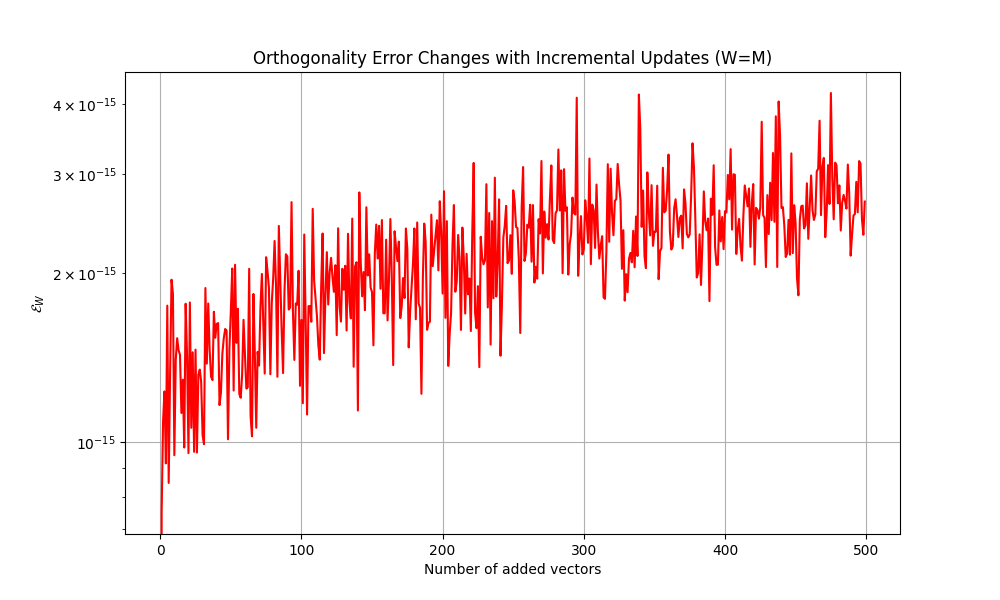
\includegraphics[width=0.7\textwidth]{../figure/simple_orthogonality_error.png}
\caption{加权正交性误差 $\mathcal{E}_W(Q)$ 随更新步数的变化（$W=M$）}
\label{fig:simple_orth}
\end{figure}

可见, 在整个500次更新过程中, $\mathcal{E}_W(Q)$ 始终维持在 $10^{-15}$ 量级（机器精度附近）, 未出现累积发散.这说明累积更新策略（式~\eqref{eq:agg_update}）从根本上避免了小正交矩阵连乘带来的误差放大 \cite{zhang2022,brand2006}.

\subsubsection{分解正确性验证}
构造一个简单的二维椭圆方程（系数 $a=1$, 源项 $f=1$, 网格尺寸 $0.1$, 有限元阶数2）验证改进ISVD输出分解的正确性.图~\ref{fig:simple_solution} 展示了有限元解在网格点上的分布.

\begin{figure}[H]
\centering
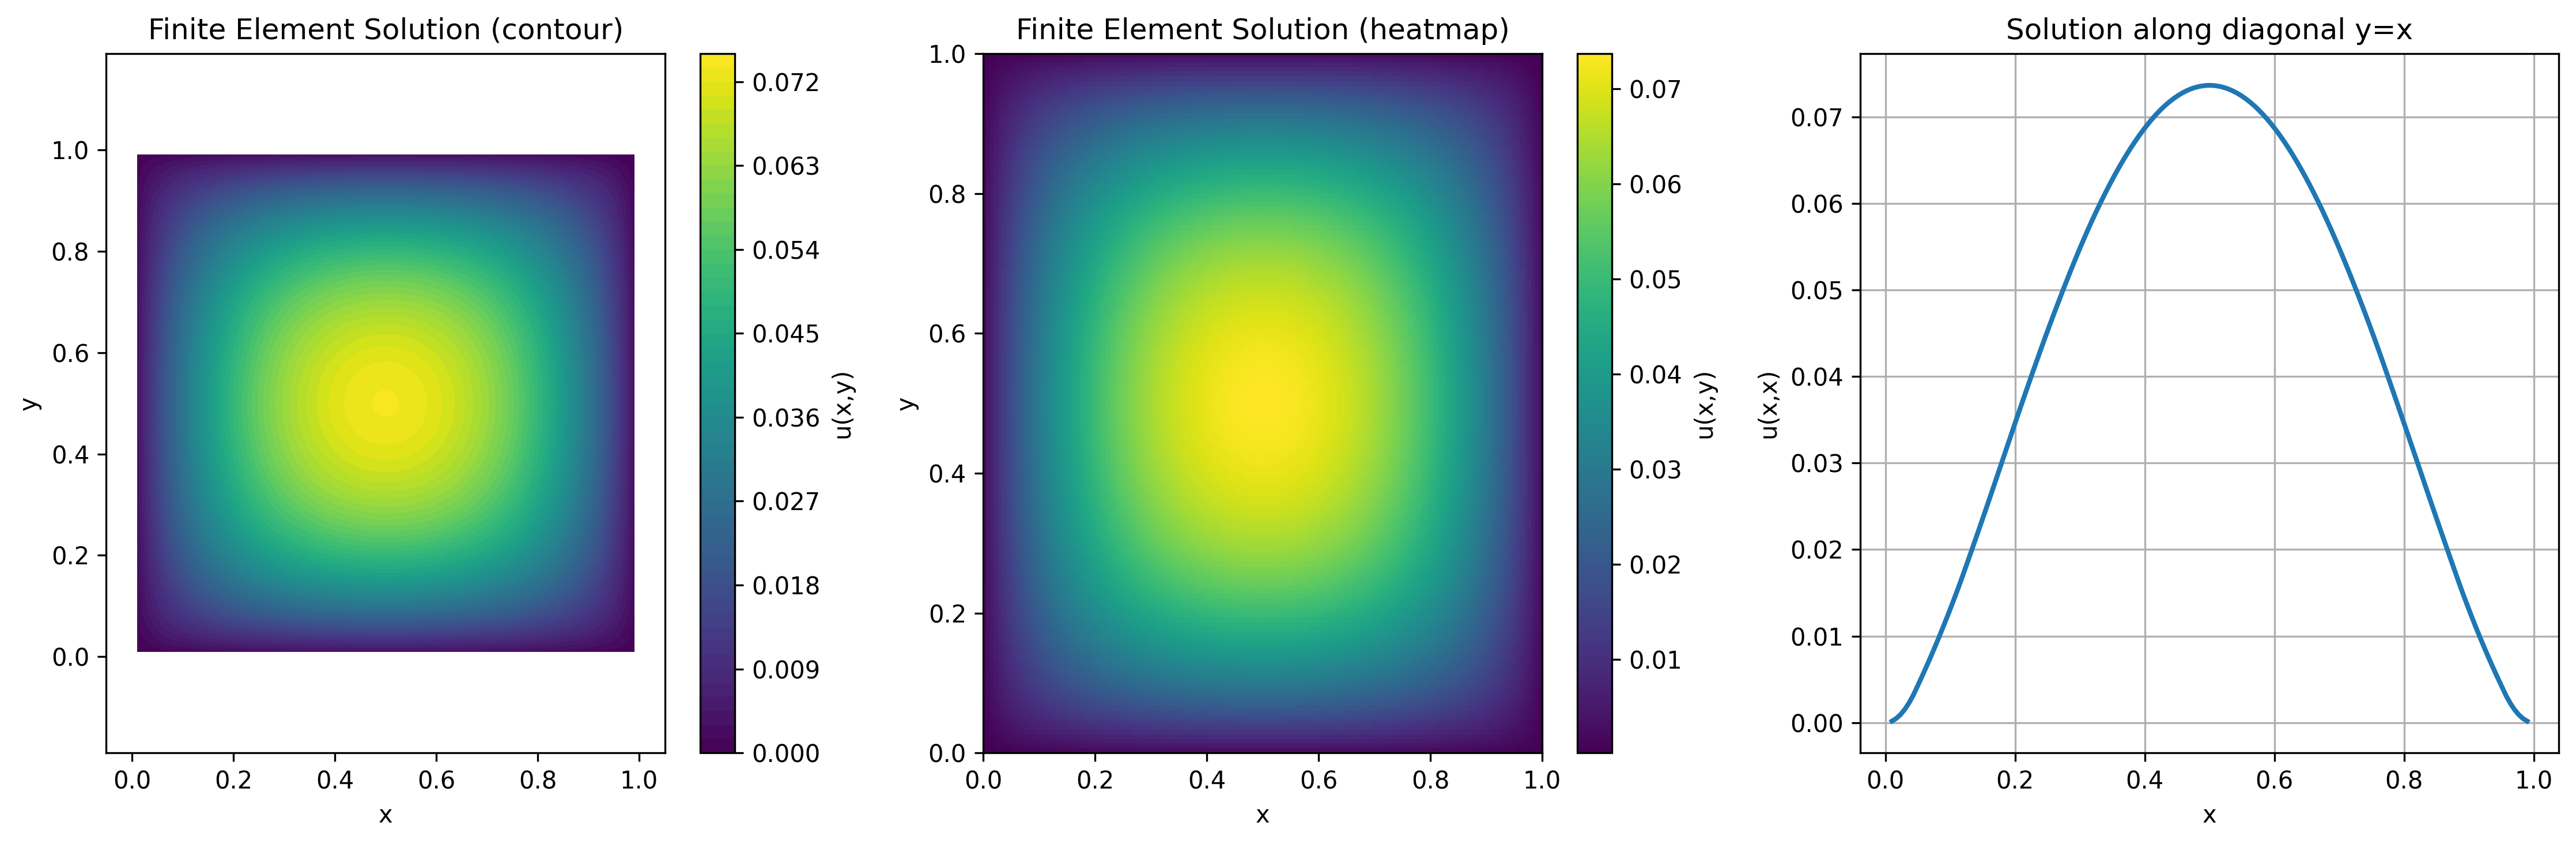
\includegraphics[width=0.6\textwidth]{../figure/simple_solution.png}
\caption{简单二维椭圆方程的有限元解分布}
\label{fig:simple_solution}
\end{figure}

进一步观察增量更新过程中核心矩阵的奇异值分布（图~\ref{fig:simple_singular_values}）, 绝大多数奇异值处于 $10^{-15}$ 量级, 表明数值秩已被有效控制, 从侧面验证了改进ISVD的数值稳定性.

\begin{figure}[H]
\centering
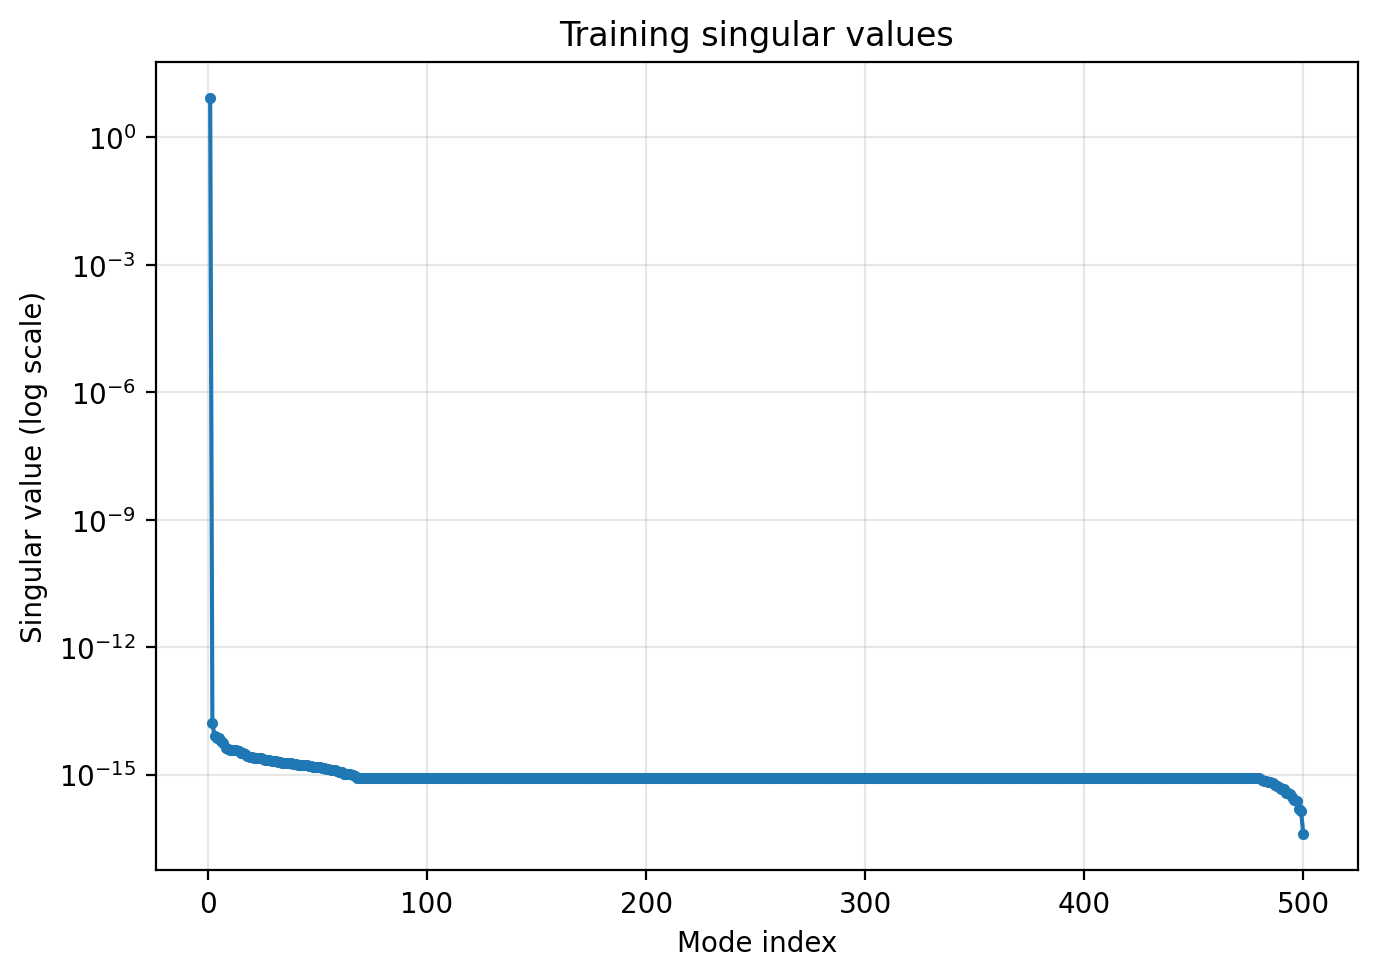
\includegraphics[width=0.7\textwidth]{../figure/singular_values.png}
\caption{核心矩阵的奇异值分布（对数坐标）}
\label{fig:simple_singular_values}
\end{figure}

\subsection{1D参数化PDE实验}

考虑一维变系数椭圆方程：
\[
-\frac{d}{dx}\bigl((1+\mu x)\frac{du}{dx}\bigr)=1,\quad x\in(0,1),\ u(0)=u(1)=0,
\]
参数 $\mu\in[0,1]$, 等距取200个训练参数, 100个测试参数.有限元离散单元数 $N=500$.

\subsubsection{离线构基时间对比}
图~\ref{fig:1d_time} 给出了批次SVD与经典Brand ISVD的累计时间随快照数增长的变化, 以及Brand ISVD的矩阵正交性误差 $\mathcal{E}_W(Q)$ 的演化.

\begin{figure}[H]
\centering
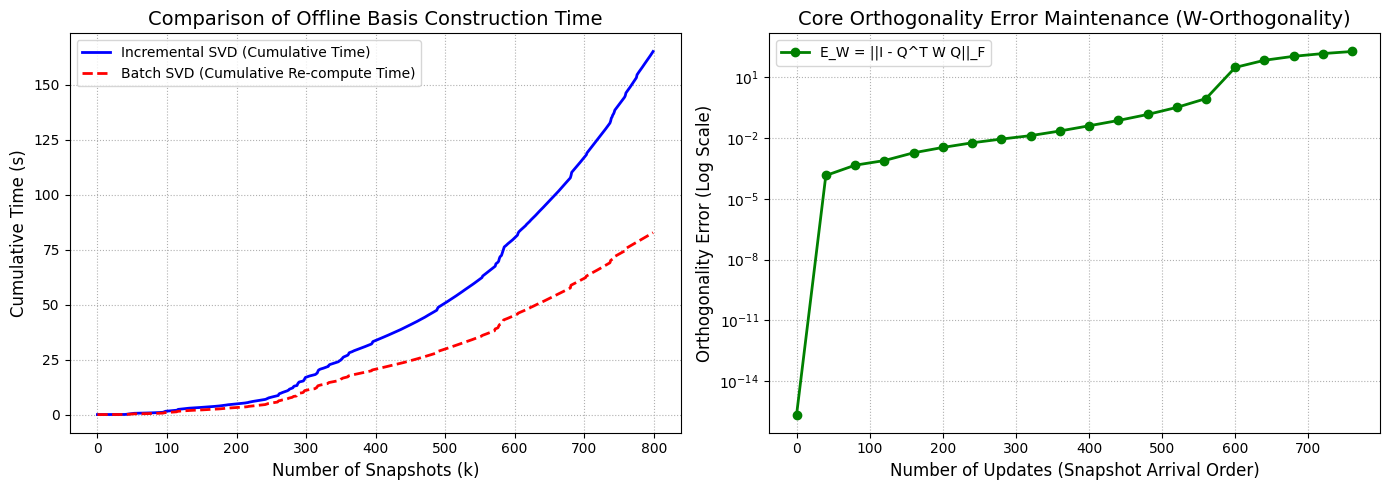
\includegraphics[width=0.7\textwidth]{../figure/1D.png}
\caption{1D问题累计离线时间对比}
\label{fig:1d_time}
\end{figure}

批次SVD的累计时间随快照数呈二次增长（$\mathcal{O}(n^2)$）\cite{golub2013matrix}；而经典Brand ISVD的累计时间增长更快, 其原因包括截断秩设置过小及Python SVD库的小矩阵开销.尤为值得注意的是, 400次更新后Brand ISVD的加权正交性误差 $\mathcal{E}_W(Q)$ 急剧上升至 $10^1$ 量级, 导致数值不稳定, 后续更新需花费更多时间处理误差 \cite{brand2006}.

\subsubsection{正交性对比}
图~\ref{fig:1d_orth} 展示了Zhang改进ISVD在运行过程中加权正交性误差的变化, 同时以批次SVD的正交性（恒为机器精度）作为基准.

\begin{figure}[H]
\centering
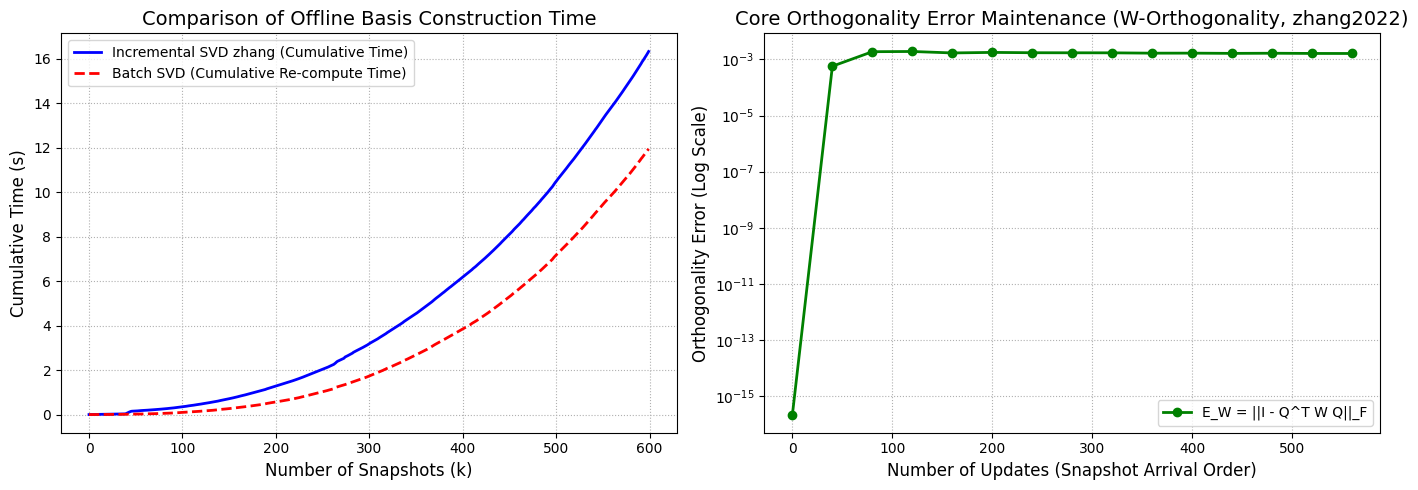
\includegraphics[width=0.7\textwidth]{../figure/1D_zhang.png}
\caption{Zhang改进ISVD的加权正交性误差}
\label{fig:1d_orth}
\end{figure}

可以看到, Zhang改进ISVD在整个550次更新中 $\mathcal{E}_W(Q)$ 始终保持在 $10^{-3}$ 以下, 远优于经典Brand ISVD在400步后的完全发散.$10^{-3}$ 的误差是算法为换取极高效率而主动付出的轻微代价, 在实际降阶应用中仍可接受.

\subsubsection{单步时间差分析}
图~\ref{fig:1d_time_diff} 给出了每次迭代中批次SVD与Zhang ISVD的单步时间差及二次拟合曲线.

\begin{figure}[H]
\centering
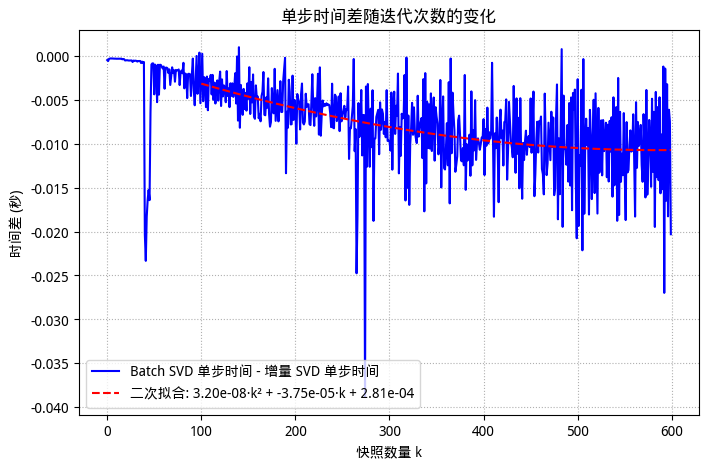
\includegraphics[width=0.7\textwidth]{../figure/1D_zhang_time.png}
\caption{单步时间差随快照数的变化（批次SVD减增量SVD）}
\label{fig:1d_time_diff}
\end{figure}

拟合曲线为 $3.20\times10^{-8}k^2 - 3.75\times10^{-5}k + 2.81\times10^{-4}$.这里的 $k$ 是当前快照数.可以看出, 单步时间差呈现二次增长趋势, 且在截断误差取机器误差时增量SVD的效率优势不明显.
所以在下面的2D大规模PDE实验中, 我们将适当放宽截断误差要求, 以更明显地展示增量SVD在大规模问题中的效率优势.


\subsection{基于两个参数的大规模PDE实验}
将模型简化为仅含线性依赖的扩散系数：
\[
-\nabla\cdot\bigl((1+\mu_1 x + \mu_2 y)\,\nabla u\bigr)=1,\quad (x,y)\in(0,1)^2,
\]
齐次 Dirichlet 边界条件.采用相同的 $40\times40$ 网格（$N=1600$）, 总快照数 $n=50\,000$, 截断秩根据奇异值阈值动态选择.参数 $\mu_1,\mu_2$ 在 $[-0.2,0.2]$ 内均匀采样.

图~\ref{fig:2d_performance_mu1mu2} 展示了 Batch SVD 与 Zhang 增量 SVD 在该简化模型上的性能对比.

\begin{figure}[H]
\centering
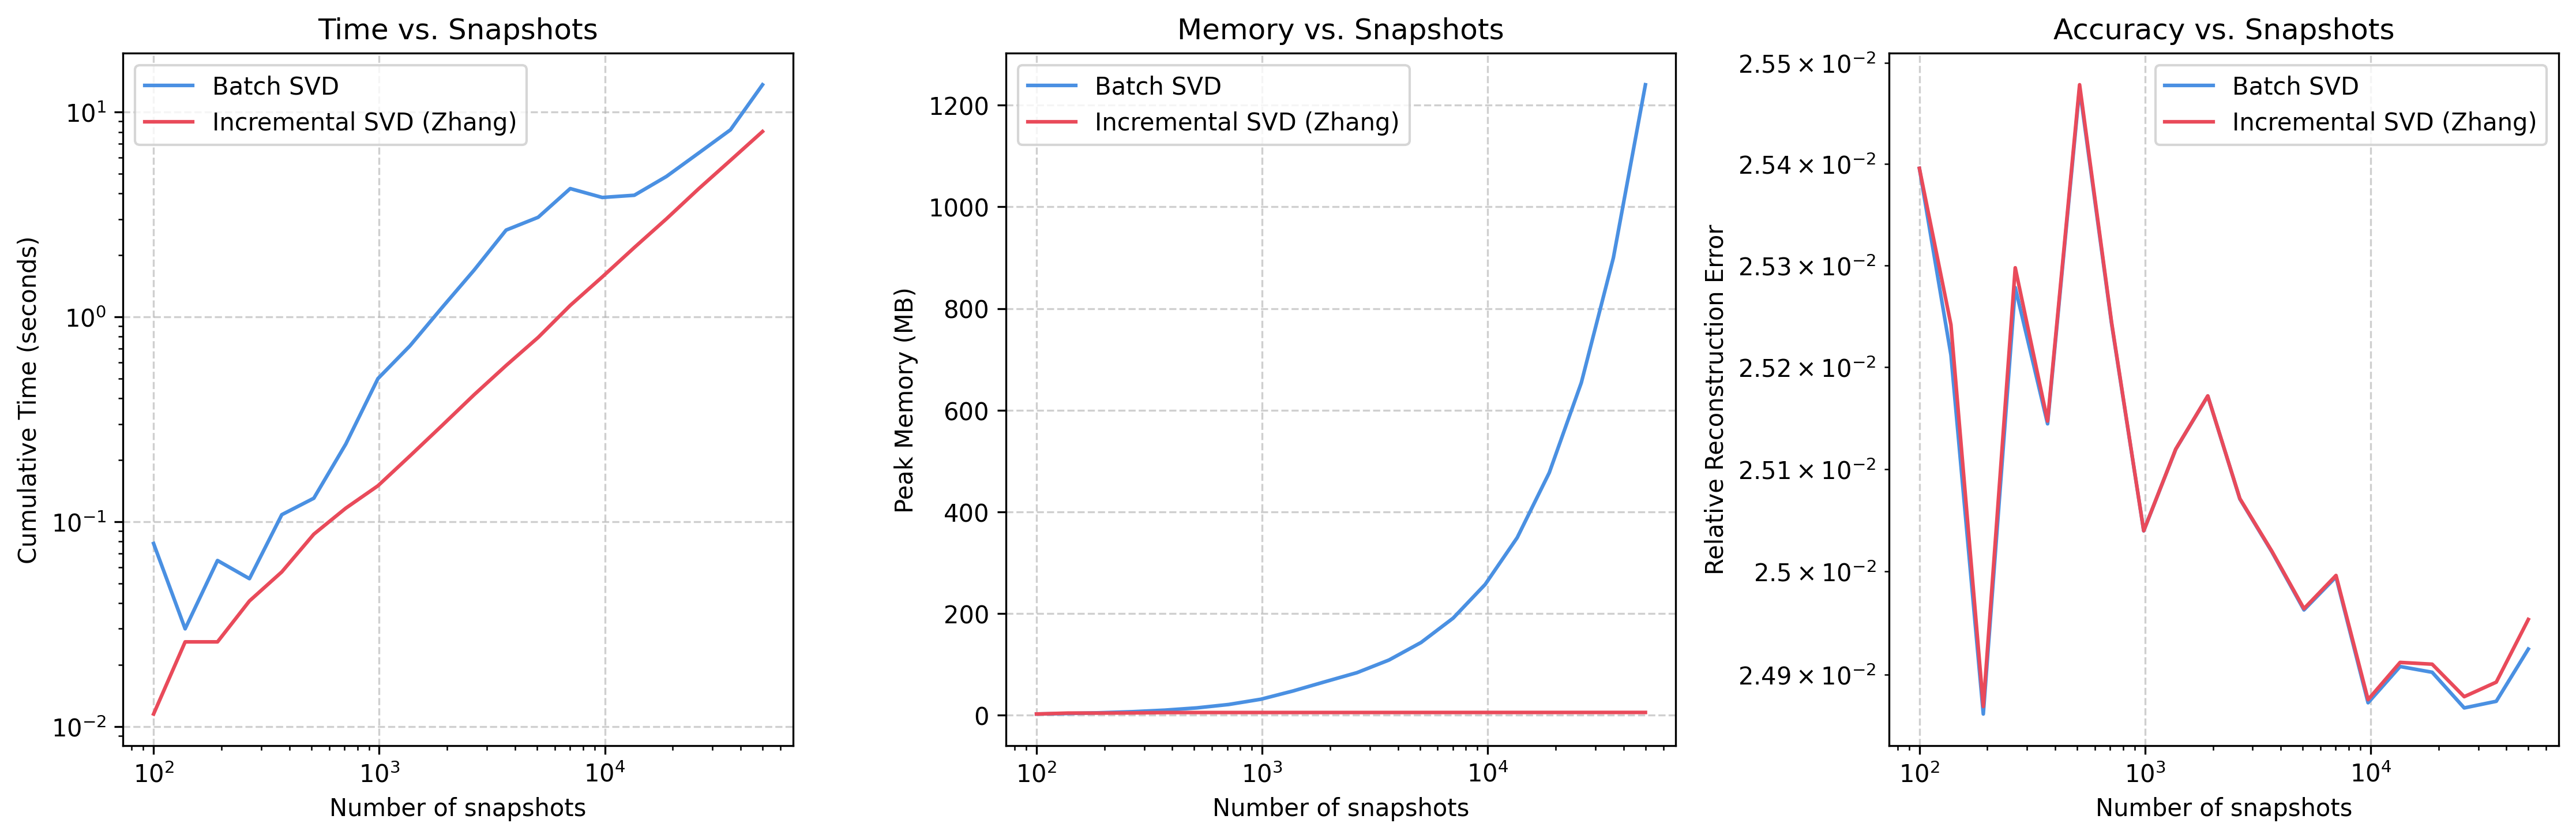
\includegraphics[width=0.9\textwidth]{../figure/svd_vs_snapshots_adaptive_r.png}
\caption{无交叉项模型下 Batch SVD 与增量 SVD 的性能对比}
\label{fig:2d_performance_mu1mu2}
\end{figure}

\textbf{内存压缩效果：}
与三个参数的模型类似, Batch POD 需要存储全部快照, 峰值内存随快照数线性增长, 当 $n=50\,000$ 时达到约 $1240$ MB.而增量 SVD 仅维护低维分解因子, 峰值内存稳定在 $10$ MB 左右, 压缩比超过 $120$ 倍, 存储节约率超过 $99\%$.

\textbf{离线时间对比：}
Batch SVD 的累计时间相对较高, 而增量 SVD 的累计时间近似线性（约 $8$ 秒）, 流式更新策略显著降低了重复计算成本.

\textbf{数值解验证：}
二者的误差几乎相差无异, 均在 $10^{-2}$ 量级, 说明增量 SVD 在保持数值稳定的同时, 能够高效逼近最优低维子空间.


\subsection{基于三个参数的大规模PDE实验}

将模型扩展至二维单位正方形区域：
\[
-\nabla\cdot((1+\mu_1 x + \mu_2 y + \mu_3 x y)\,\nabla u)=1,\quad (x,y)\in(0,1)^2,
\]
齐次Dirichlet边界条件.采用 $40\times40$ 的网格剖分, 自由度 $N=1600$, 总快照数 $n=50\,000$, 截断秩根据奇异值阈值动态选择.
\begin{figure}[H]
\centering

\includegraphics[width=0.9\textwidth]{../figure/svd_vs_snapshots.png}
\caption{Batch SVD与增量SVD的性能对比：累计时间、峰值内存及重建误差随快照数的变化}
\label{fig:2d_performance}
\end{figure}

\textbf{离线时间对比：}
与之前两个参数的大规模PDE结果相仿, Batch POD的累计时间随快照数呈超线性增长（最终为12.39秒）, 这是由于每次完整SVD的代价随矩阵规模增大而急剧增加.相比之下, Zhang ISVD的累计时间近似线性增长（最终为8.43秒）, 其增量更新策略避免了重复处理历史数据.尽管在快照数较小时增量SVD的单块开销略高, 但随着数据量增大, 其流式计算的优势愈发明显.

\textbf{内存压缩效果：}
这里和两个参数的实验相差不大.Batch POD需要同时存储所有历史快照, 当快照数达到50000时, 峰值内存高达1240.3 MB（存储整个快照矩阵）.而Zhang ISVD采用流式处理, 仅保留低维分解因子 $(Q,\Sigma,R)$, 峰值内存稳定在10.3 MB, 压缩比达到120倍.即使与完整存储所有快照的Batch POD相比, 增量方法的存储节约率也达到99.17\%, 充分体现了其在大规模快照数据下的内存优势.

\textbf{数值解验证：}
图~\ref{fig:2d_performance} 中的误差子图展示了两种方法重建快照矩阵的相对误差.Batch POD的重建误差稳定在约 $2.1\times10^{-7}$, 而Zhang ISVD的误差从初始的$2.00\times10^{-7}$的机器误差变化到 $6.77\times10^{-2}$, 之后迅速下降, 最终收敛到 $1.47\times10^{-5}$.这表明增量SVD在流式处理过程中能够高效逼近最优低维子空间, 且最终精度满足工程需求.若需要与高精度有限元解进行点对点对比, 以测试参数 $\mu=0.5$ 为例, 降阶解的最大相对误差约为 $10^{-5}$ 量级, 说明截断后的低维基足以捕捉主导物理特征 \cite{hesthaven2015,patera_rozza}.

\section{结论与未来展望}

\subsection{结论}

通过一维和二维参数化椭圆型方程的数值实验, 我们对增量奇异值分解在缩减基构造中的表现有了一些认识.

先看数值稳定性, 实验中发现, 它确实避免了Brand算法随着更新步数增加正交性变差的问题.不过有意思的是, 在二维大规模算例中, 增量SVD的最终重建误差稳定在$1.5\times10^{-5}$左右, 而批处理SVD可以做到$2.1\times10^{-7}$.两者差了两个数量级.虽然对于工程问题这个精度通常够用了（比如$10^{-5}$对解场来说已经很不错）, 但这个差距还是值得注意的.增量方法的初始误差一度跳到$6.77\times10^{-2}$, 随着快照增加才慢慢降下来.这说明刚起步的几块数据质量对整体影响比较大.

内存方面的收益非常明显.在$40\times40$网格、五万快照的设定下, 普通批处理SVD要存下整个快照矩阵, 峰值内存跑到1240.3MB.增量SVD只需要维护低维分解因子, 稳定在10.3MB, 压缩比超过120倍, 节省了99\%以上的内存.这意味着即使快照数量再翻几倍, 内存也不至于成为瓶颈.

计算时间上, 批处理SVD累计花了12.39秒, 增量SVD是8.43秒, 快了大概三分之一.而且增量SVD基本是线性增长.虽然处理小块数据时增量SVD的单块开销比批处理高一点, 但快照一多, 流式更新的好处就显现出来了.

总的来说, 对于快照量很大的离线构基任务, 增量SVD在内存、时间、精度之间找到了一个很实用的平衡点, 尤其是在内存受限的场景下, 它比传统的批处理SVD更合用.

\subsection{未来展望}

尽管增量SVD在数值实验中表现出良好的性能, 仍有若干理论问题需要进一步澄清.首先, 精度损失的内在机理尚不明确.增量SVD的最终重建误差收敛至$10^{-5}$量级, 而批处理SVD可达$10^{-7}$, 两者之间存在约两个数量级的差距.这一误差的来源需从累积更新过程的各个环节加以分析, 特别是投影残差、QR分解以及局部SVD截断对整体精度的影响.此外, 块大小与截断阈值对误差的定量影响关系尚未建立.若能从理论上推导出误差的上界, 将为实际应用中的参数选择提供重要依据.

其次, 当前实验仅覆盖了自由度$N=1600$、快照数$n=50\,000$的规模.对于真实工程问题, 如三维非定常流动或全阶模型自由度达数十万乃至上百万、快照数达百万量级的场景, 增量SVD的可扩展性仍需验证.具体而言, 需要考察其在超大规模下是否仍能保持近似线性的计算时间增长, 以及是否能够在分布式内存或磁盘流式存储的条件下高效运行.

另外, 现有算法采用固定的块大小和固定的截断阈值, 缺乏自适应性.未来可探索根据新快照与当前低维子空间之间的残差范数动态调整更新频率, 或根据奇异值谱的衰减速率自动选择截断精度.这种自适应策略有望在计算开销与近似精度之间实现更优的权衡.

最后, 增量SVD可与更完整的模型降阶流程深度集成.例如, 将其与贪婪采样方法或在线后验误差估计器相结合, 实现“边采样边构基”的完全在线离线构基模式.这一方向有望进一步提升many-query场景下的整体计算效率.

综上所述, 增量SVD在工程降阶中的应用仍有诸多值得深入研究的理论缺口与技术细节.填补这些空白, 将有助于将其从一种启发式算法发展为具有严格理论保证且适用于大规模计算的标准工具.